\chapter{Background and Challenges in GANs}
%\epigraph{\itshape  La volonté trouve, la liberté choisit. Trouver et choisir, c'est penser}{-- Victor Hugo}

\startcontents[chapters]

\printmyminitoc{
Understanding the fundamental challenges in GAN training requires a solid grasp of their core architecture and mathematical foundations. This chapter introduces the basic GAN framework and examines the key obstacles that have motivated decades of research improvements. We focus on the mathematical properties of the original GAN objective function that lead to training instability and mode collapse, providing the essential background for understanding the solutions presented in Chapter 2.
}

\fancyhead[LE]{\textsc{\chaptername~\thechapter}}

\section{Fundamentals of Generative Adversarial Networks}

\subsection{GAN Architecture and Mathematical Framework}

Generative Adversarial Networks (GANs), introduced by Goodfellow in 2014 \cite{ref1}, consist of two neural networks—a generator (G) and a discriminator (D)—that compete in a zero-sum game. The generator learns to produce synthetic data that mimic real samples, while the discriminator attempts to distinguish between real and generated data. This adversarial process drives both networks to improve iteratively, pushing the generator to create increasingly realistic outputs.

\begin{figure}
    \centering
    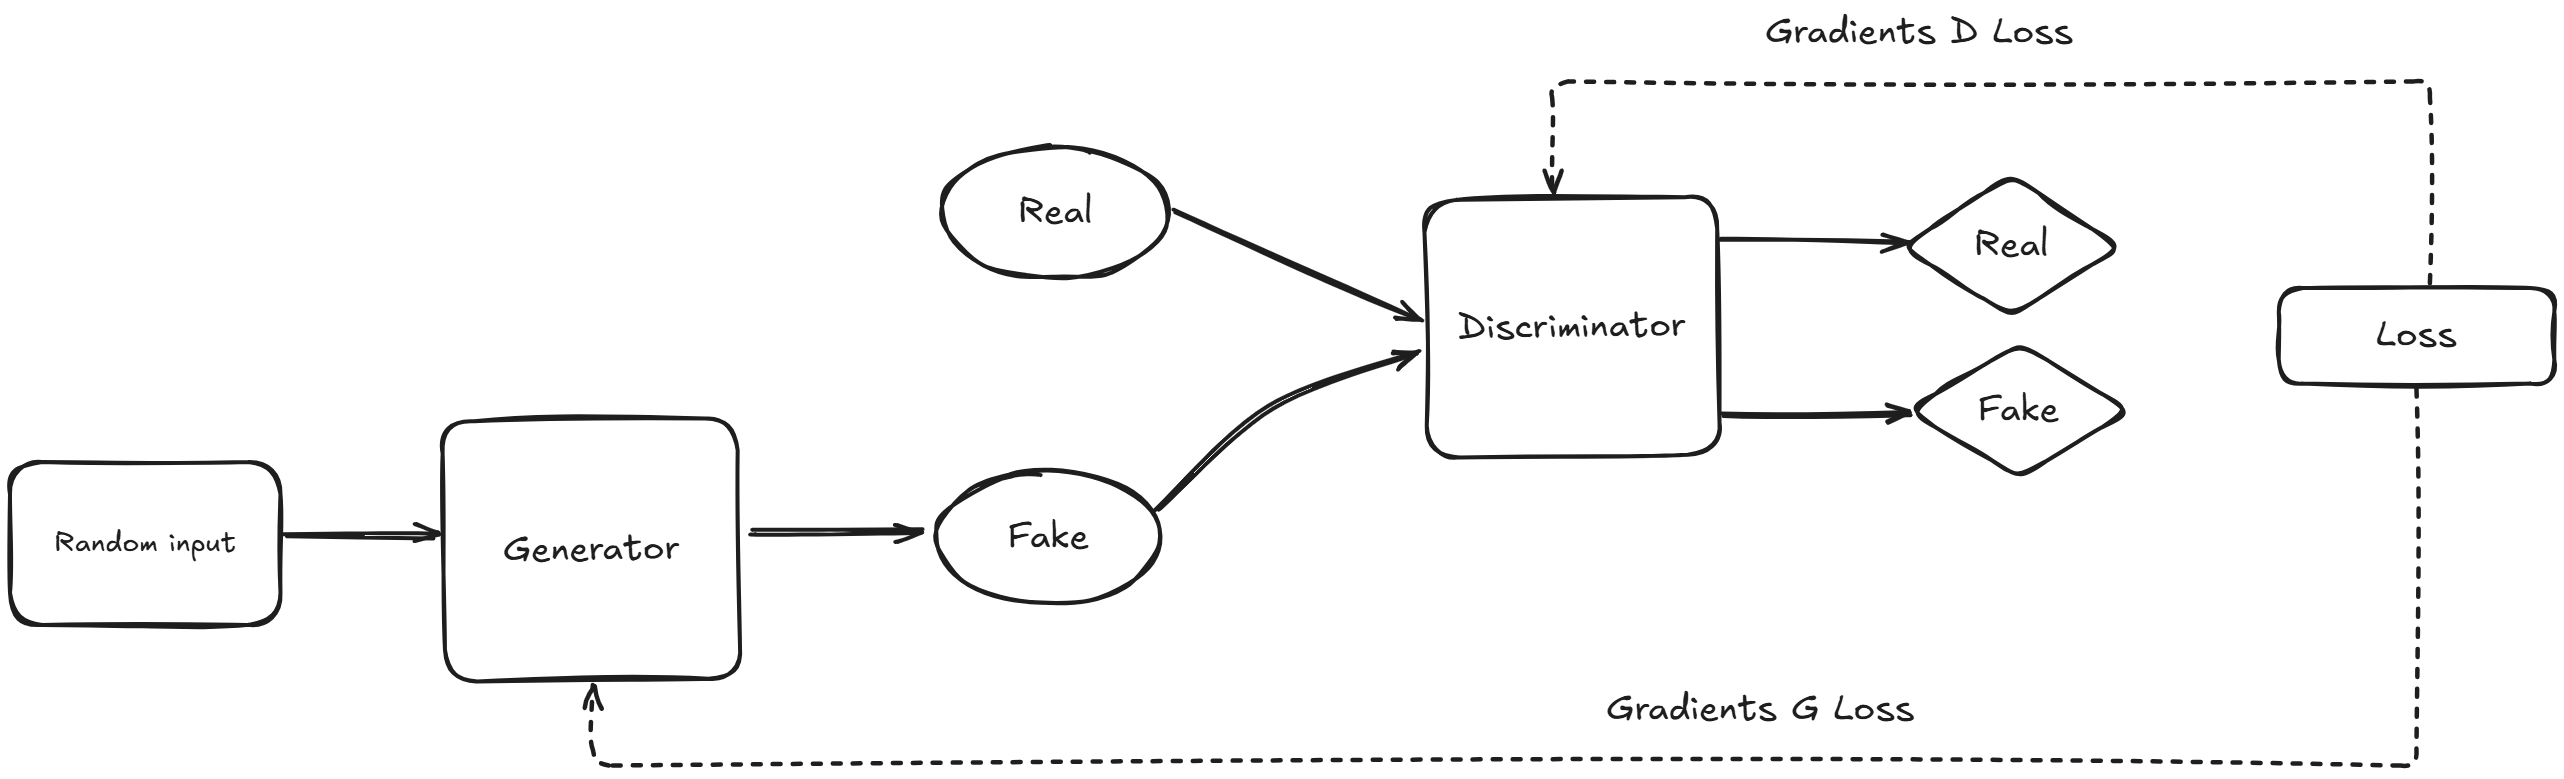
\includegraphics[height=5cm]{images/GAN_Core.png}
    \caption{Generative Adversarial Networks Core}
    \label{fig:enter-label}
\end{figure}

The objective function formalizes this competition as a minimax game where the discriminator $D$ and generator $G$ have opposing goals.\cite{goodfellow2014generative}  The discriminator seeks to maximize its ability to correctly classify real samples (drawn from the true data distribution $p_{\text{data}}$) as real and generated samples $G(z)$ as fake. Conversely, the generator aims to minimize the discriminator's success rate by producing increasingly realistic synthetic data that can fool the discriminator.

\begin{equation}
    \min_G \max_D \mathbb{E}_{x \sim p_{\text{data}}} \left[ \log D(x) \right] + 
    \mathbb{E}_{z \sim p_z} \left[ \log (1 - D(G(z))) \right].
\end{equation}

Here:
\begin{itemize}
    \item $p_{\text{data}}$ represents the true data distribution from which real samples are drawn.
    \item $x \sim p_{\text{data}}$ denotes a real sample $x$ sampled from the data distribution.
    \item $p_z$ is a prior distribution (e.g., Gaussian or uniform) from which the generator samples latent noise vectors.
    \item $z \sim p_z$ represents a noise vector $z$ sampled from the prior distribution.
    \item $G(z)$ generates synthetic data by mapping the latent noise vector $z$ to the data space.
    \item $D(x)$ outputs the probability that a given sample $x$ comes from real data rather than the generator (i.e., $D(x) \in [0,1]$ where values close to 1 indicate "real" and close to 0 indicate "fake").
    \item $\mathbb{E}_{x \sim p_{\text{data}}}[\cdot]$ denotes the expected value over samples drawn from the true data distribution.
    \item $\mathbb{E}_{z \sim p_z}[\cdot]$ denotes the expected value over noise vectors drawn from the prior distribution.
\end{itemize}

\subsection{Theoretical Foundations and Optimal Discriminator}

When the discriminator reaches its optimal form $D^*$, the generator's objective becomes equivalent to minimizing the Jensen-Shannon (JS) divergence between the real and generated distributions. \cite{goodfellow2016tutorial} The Jensen-Shannon divergence is defined as:

\begin{equation}
JS(P_r, P_g) = \frac{1}{2}KL(P_r \| P_m) + \frac{1}{2}KL(P_g \| P_m)
\end{equation}

where $P_m = \frac{P_r + P_g}{2}$ is the mixture distribution, and $KL$ denotes the Kullback-Leibler divergence:
\begin{equation}
KL(P \| Q) = \mathbb{E}_{x \sim P}\left[\log\frac{P(x)}{Q(x)}\right]
\end{equation}

Under an optimal discriminator $D^*$, the generator's loss becomes:
\begin{equation}
\min_G \mathbb{E}_{x \sim p_{data}}[\log D^*(x)] + \mathbb{E}_{z \sim p_z}[\log(1-D^*(G(z)))] = 2 \cdot JS(P_r, P_g) - 2\log 2
\end{equation}

This minimax formulation ensures that as training progresses, the generator becomes increasingly skilled at producing realistic data while the discriminator becomes better at detecting subtle differences between real and synthetic samples, driving both networks toward an optimal equilibrium. However, this mathematical relationship reveals a fundamental limitation that leads to the training challenges discussed in the following section.

\section{Critical Training Challenges}

\subsection{Mode Collapse}

Mode collapse represents one of the most critical obstacles in effectively training Generative Adversarial Networks (GANs), as it hinders the ability of the model to generate diverse, high-quality outputs and achieve stable convergence\cite{goodfellow2016tutorial}.

\textbf{Mode collapse} is a significant issue in the training of Generative Adversarial Networks (\textsc{gan}s), where the generator fails to produce a diverse range of outputs, often cycling between a few modes without capturing the full variety of the target data distribution. This problem arises due to the nature of the optimization in GANs, which can lead the generator to focus on a limited set of modes during training, rather than capturing all the modes of the target distribution.

A key driver of mode collapse lies in the distinction between the minimax and maximin formulations of the GAN objective. In the ideal minimax formulation:

\begin{equation}
    G^* = \min_G \max_D V(G, D),
\end{equation}
the generator \(G\) converges to the true data distribution when optimized against an optimal discriminator \(D\). However, in practice, simultaneous gradient descent often behaves like the maximin formulation:
\begin{equation}
    G^* = \max_D \min_G V(G, D),
\end{equation}
During the inner-loop minimization over \(G\) , the generator is pressured to map distinct latent vectors \(z\) to identical outputs \(x\) that the discriminator \(D\) cannot reliably classify as fake. This creates an incentive for \(G\) to exploit 'safe' outputs that consistently fool \(D\), causing it to abandon diversity and focus on a narrow subset of modes in the data distribution.

\subsection{Training Instability and Non-convergence}

Generative Adversarial Networks (GANs) often suffer from \textbf{instability} and \textbf{non-convergence} during training, largely due to the nature of their adversarial optimization process. \cite{salimans2016improved, arjovsky2017principled} The generator \( G \) typically uses one of two loss functions:  

\begin{equation}
    J_G = - \mathbb{E}_{z} [\log D(G(z))]
\end{equation}
or
\begin{equation}
J_G = - \mathbb{E}_{z} [\log(1 - D(G(z)))]
\end{equation}

Both formulations suffer from \textbf{vanishing gradients} when the discriminator \(D\) becomes too confident in its predictions. For instance, if 

\begin{equation}
D(G(z)) \to 0 \quad \text{(i.e., \(D\) perfectly identifies generated samples)},
\end{equation}

the gradient $\nabla$ of \(J_G\) with respect to \(G\)'s parameters diminishes:

\begin{equation}
\nabla_G J_G \to 0 \quad \text{as} \quad D(G(z)) \to 0
\end{equation}

halting \(G\)'s progress. Conversely, if 

\begin{equation}
D(G(z)) \to 1 \quad \text{(generated samples completely fool \(D\))},
\end{equation}

then:

\begin{equation}
\nabla_G J_G \to 0 \quad \text{as} \quad D(G(z)) \to 1
\end{equation}

meaning the generator receives no meaningful update signal. This \textbf{asymmetry} destabilizes training, as minor imbalances in \(G\) and \(D\)'s learning rates can lead to divergent behavior rather than cooperative optimization.